\documentclass[11pt, a4paper, oneside]{article}   	% use "amsart" instead of "article" for AMSLaTeX format
%\usepackage{geometry}                		% See geometry.pdf to learn the layout options. There are lots.
%\geometry{letterpaper}                   		% ... or a4paper or a5paper or ... 
%\geometry{landscape}                		% Activate for for rotated page geometry
%\usepackage[parfill]{parskip}    		% Activate to begin paragraphs with an empty line rather than an indent

\usepackage{fancyhdr} % En-tᅵᅵte et pieds de page
\usepackage{lastpage} % Definition 1ᅵᅵre et derniᅵᅵre page

\usepackage[utf8]{inputenc}
\usepackage[T1]{fontenc}
\usepackage[french]{babel}

\usepackage{graphicx}% Pour les images
\usepackage{array}% Tableau si besoin
\usepackage{lscape}%Format paysage si besoin
\usepackage{hyperref} % Pour crᅵᅵŽer des lien hypertexts: \url{my_url}
\usepackage{multirow}
\usepackage{amsmath} % Equation non numᅵᅵŽrotᅵᅵŽe et autres
\usepackage{esint} % double, triple integrals
\usepackage{amssymb}
\usepackage{array}
\usepackage{numprint}
\usepackage{dsfont} % Ensembles C,R,N ,...
\usepackage[margin=3.0cm]{geometry} % Marges$
\usepackage[squaren,Gray,cdot]{SIunits} % Pour les unitᅵᅵŽs (cf http://fr.wikibooks.org/wiki/LaTeX/%C3%89crire_de_la_physique) \unit{nombre}
\usepackage{caption}
\usepackage{subcaption}
\usepackage{wrapfig}%permet de mettre image bloc

\usepackage{tikz}%symbole check \checkmark

\usepackage{pdfpages}%pfd usage
\usepackage{float}%place les image où on veut !

% Section new page
\newcommand{\sectionbreak}{\clearpage}%c'est top !!
 
\pagestyle{fancy}
\fancyhf{}
\rhead{\leftmark}
\lhead{Projet de Programmation}
\rfoot{Page \thepage}
\lfoot{ \vspace{0.1cm}\begin{picture}(0,0) \put(0,0){
\includegraphics[width=2cm]{images/epfl-logo.eps}} \end{picture}}%\vspace{0.1cm}\begin{picture}(0,0) \put(0,0){
\includegraphics[width=2cm]{images/epfl-logo.eps}} \end{picture}}


%Page de titre
\title{Projet de programmation \\ \vspace{+100pt}\textbf{D'une photo d'un graphe à un graphique numérique}}
 
\author{\vspace{+300pt}\\ Groupe composé de \vspace{+10pt} \\Julien Rey \\Jonathan Burkhard}
\date{\vspace{+10pt}
%Logo de EPFL
\begin{figure}[H]
\begin{center}
	
\includegraphics[scale =0.9]{images/epfl-logo.eps}
\end{center}
\end{figure}
}	
%\date{}							% Activate to display a given date or no date


%***************************************************************************************************************************
% Début du document
%***************************************************************************************************************************
\begin{document}
\maketitle
\tableofcontents
\clearpage
%***************************************************************************************************************************
% Début du texte
%***************************************************************************************************************************



%***************************************************************************************************************************
% Introduction
%***************************************************************************************************************************
\section{Introduction}

Le but de ce projet est de récupérer les points de pixel dans un fichier image et de reprendre chacun des pixels en passant par trois languages de programmation :
\begin{enumerate}
\item Labview
\item C++
\item Matlab
\end{enumerate}

Nous devrons apprendre à gérer le transfert des données entre les différentes applications ainsi que le la gestion des erreurs dans celles-ci. Comme nous étions pas sur le même système d'exploitation, nous avons écris un programme qui dépendait de la plateforme ce qui nous a permis de travailler à deux. Par la suite, nous nous sommes concentré seulement sur la plateforme de Mac en travaillant ensemble.

\section{Descriptions}

La plateforme utilisé est Mac OS avec Geany comme éditeur. La version du compilateur est gcc version 4.8.3.

Voici le schéma du déroulement du programme créé. Il permet de comprendre le rôle de chacun des sous fichiers.

\begin{figure}[H]
\begin{center}
	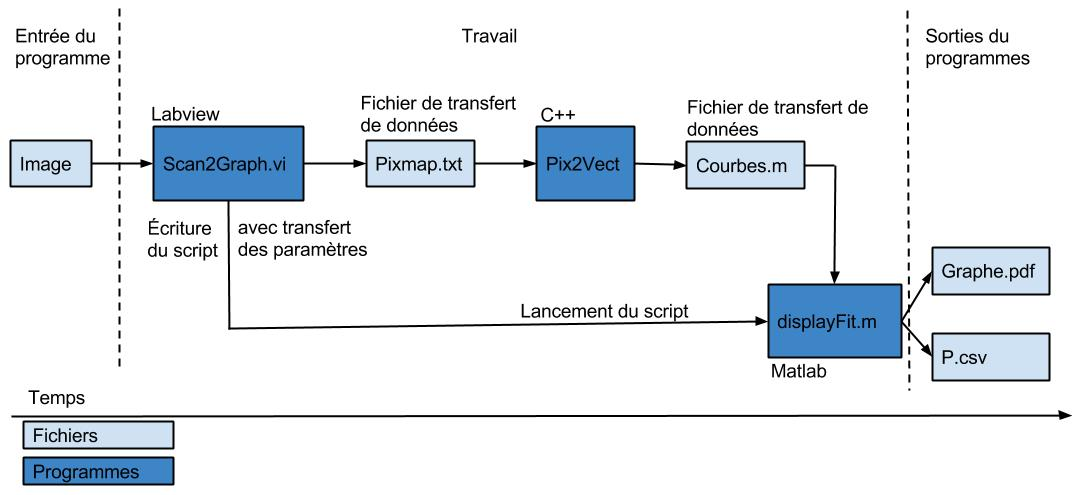
\includegraphics[scale =0.4]{images/CheminProgramme}
	\caption*{Diagramme de déroulement}
\end{center}
\end{figure}
\subsection{Fichiers}

Voici une description de chacun des fichiers contenu dans le dossier rendu.

\begin{description}
\item[$courbes.m$] Fichier écrit par le programme C++ qui contient les données du/des futur(s) graphes dans Matlab
\item[$displayFit.m$] Script écrit et lancé par Labview qui va dessiner les différentes courbes
\item[$MP\_LaunchMatlabScript.vi$] Sous-VI qui lance Matlab
\item[$P.csv$] Fichier CSV créé par Matlab qui y inscrit les coefficients des polynômes
\item[$Pix2Vect$] Executable du programme C++
\item[$Pix2Vect.cc$] Programme C++ contenant le code
\item[$Pix2Vect.o$] Compilation du programme C++
\item[$Pixmap.txt$] Fichier généré par Labview qui contient la dimension de l'image, les couleurs, et chacun des pixels
\item[$Fichier PDF$] Fichier sous plusieurs noms des graphes sortit par Matlab
\item[$Scan2graph.vi$] Programme Labview principal qui contient l'environnement graphique pour une utilisation facilitée.
\end{description}

\subsection{Procédure}
Avant tout, il faut ouvrir le fichier $Scan2graph.vi$. Après cette première étape, il est temps de choisir les différents paramètre à entrer dans l'espace Matlab afin d'y mettre ses préférences(telle que interpoler le graphe avec un polynôme du degré souhaité). Dès que cela est fait, il suffit d'appuyer sur le bouton pour lancer ou non lors de l'exécution la partie Matlab. C'et en axant la croix que le programme dessine affiche et crée les différents fichiers de sortie. \\

Ensuite, l'utilisateur doit lancer le programme en appuyant sur la flèche qui permet d'exécuter le code.
Une fois lancé, une ouverture d'un sélecteur de fichier va permettre d'ouvrir et de charger le graphique voulu et permettre de générer automatiquement le fichier $Pixmap.txt$.\\
En arrière plan, il y aura aussi la génération du script de Labview ainsi que le lancement du programme C++ qui va permettre de créer le fichier $courbes.m$.\\

Et dans un troisième temps lancer le script généré pour afficher les courbes sur un graphe de Matlab.

\subsection{Transfert de données entre les programmes}

Nous avons décidé de n'utiliser que les fichiers proposés dans la donnée pour transférer les données d'un programme à l'autre (pas de fichier temporaire supplémentaire). Les informations pour les couleurs et les types de lignes à utiliser dans Matlab passe directement avec le fichier script ($displayFit.m$).\\

Le fichier $Pixmap.txt$ est là pour transférer les données de l'image au programme C++. Il aurait pu y avoir la méthode de rentrer directement sans le fichier texte en les passant comme entrée. C'est ce que nous avons fait pour passer le système d'opération qui n'est pas dans le fichier Pixmap. Cela nous permet d'adapter le programme C++ pour la lecture des lignes qui posait posait problème sur nos deux machines.

\clearpage
%***************************************************************************************************************************
% Labview
%***************************************************************************************************************************
\section{Labview}
Nous avons écrit un programme qui permet de prendre une image, de l'afficher, d'en tirer les principale information et de les écrire dans un fichier $Pixmap.txt$.

\begin{figure}[H]
\begin{center}
	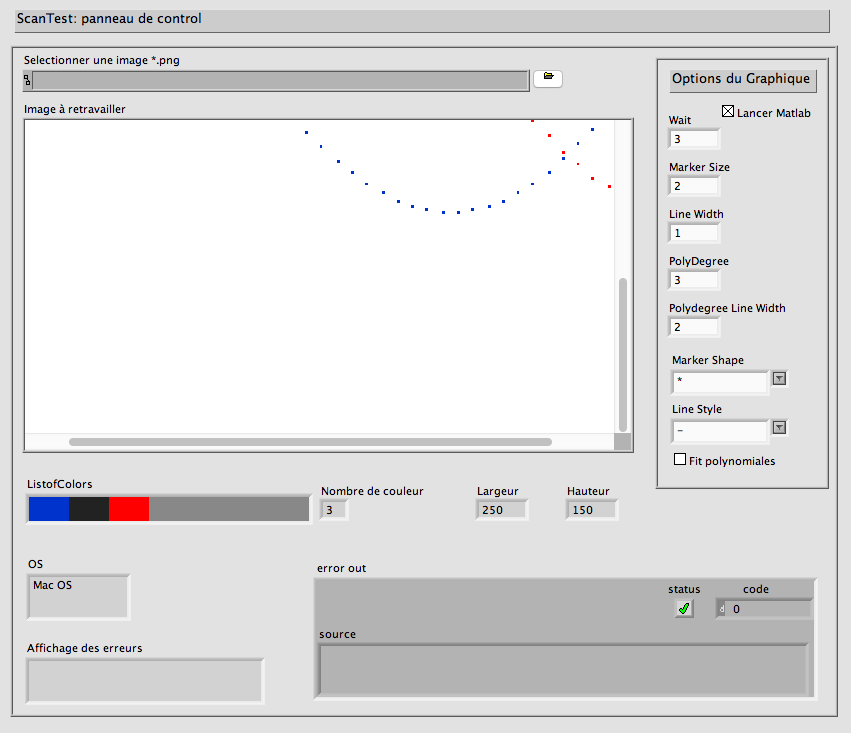
\includegraphics[scale =0.5]{images/display}
\end{center}
\end{figure}

La partie Labview est organisée en un VI principal (Scan2graph) avec un front panel (image ci-dessus) ainsi que de 3 sous VI. Le premier ($MP LaunchMatlabScript.vi$) sert à lancer Matlab et les deux autres faits sur mesure nous permette de gagner un peu de place sur le diagramme principal. Un pour afficher les vraies couleurs trouvées sur l'image et les transmettre à Matlab ($VRAI COULEUR.vi$) et l'autre pour la concaténation de la string correspondante au script Matlab ($MATLAB SCRIPT CONCAT STRING.vi$).

\begin{figure}[H]
\begin{center}
	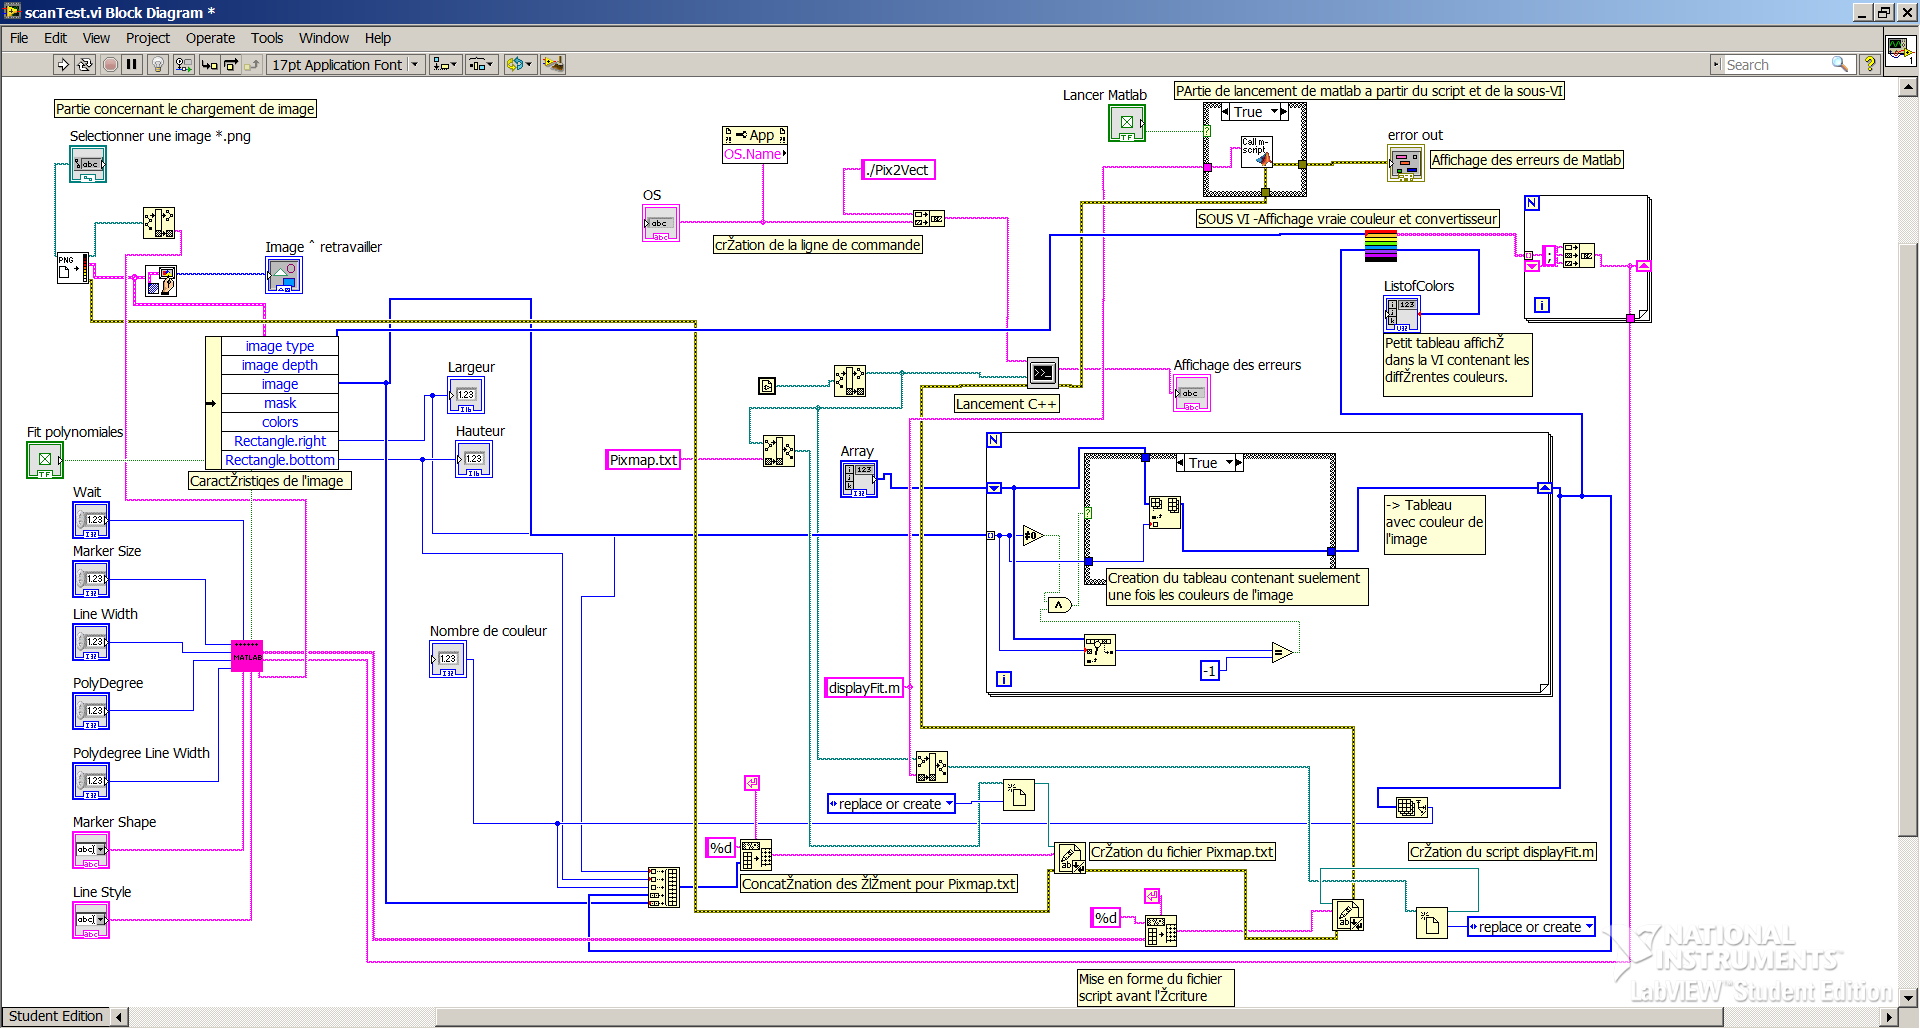
\includegraphics[scale =0.4]{images/MAIN_VI_ScanTest}
	\caption*{MAIN VI "Scan2graph"}
\end{center}
\end{figure}

\begin{figure}[H]
\begin{center}
	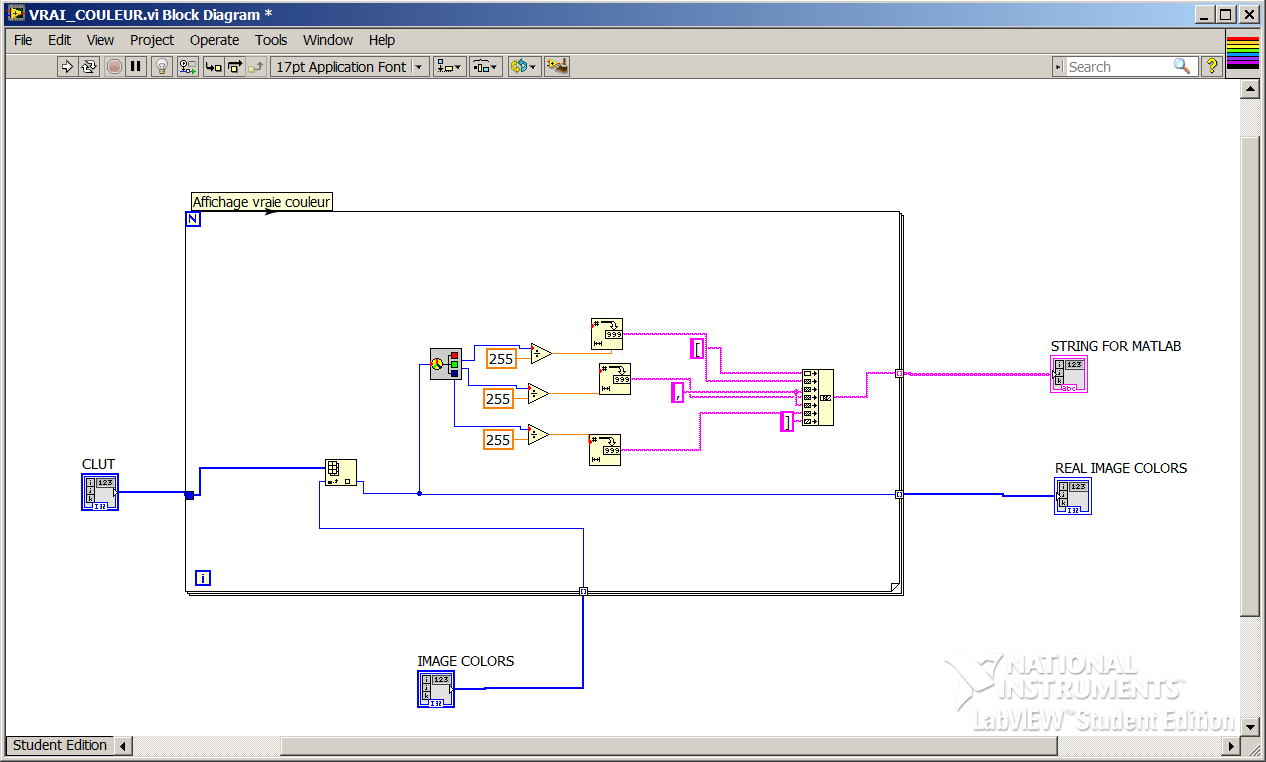
\includegraphics[scale =0.5]{images/SOUS_VI_AffichageVraiesCouleurs}
	\caption*{SOUS VI "VRAI COULEUR"}
\end{center}
\end{figure}

\begin{figure}[H]
\begin{center}
	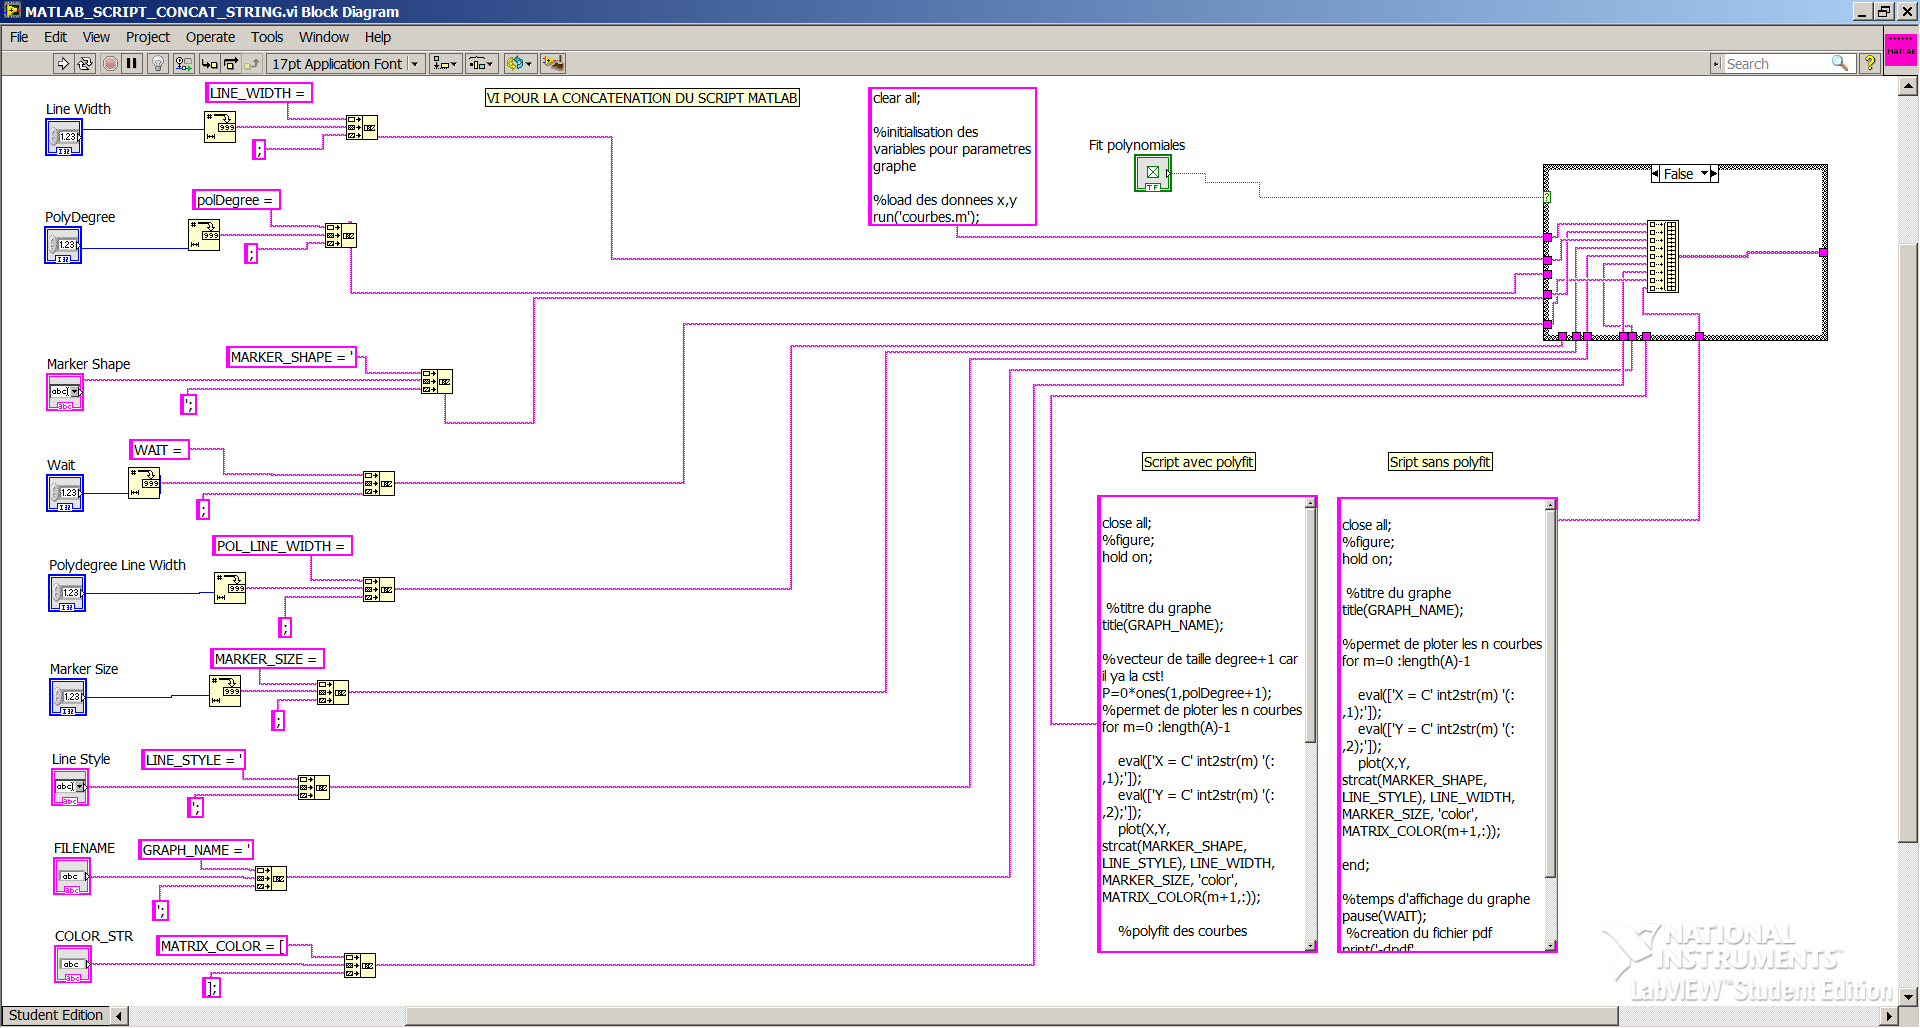
\includegraphics[scale =0.4]{images/SOUS_VI_MATLAB_SCRIPT}
	\caption*{SOUS VI "MATLAB SCRIPT CONCAT STRING"}
\end{center}
\end{figure}


\clearpage
%***************************************************************************************************************************
% C++
%***************************************************************************************************************************
\section{C++}

\subsection{$Pix2Vect.cc$}
Le programme C++ est constitué de plusieurs partir. Il a été écrit pour avoir le moins de contenu dans la main et celle-ci va tout simplement appeler un liste de fonction qui elles mêmes vont appeler d'autre fonction. Cela permet d'alléger la lecture et dans le cadre d'un programme plus lourd pouvoir réutiliser par exemple les fonctions avec d'autres arguments.\\

On a decider de créer une structure de coordonnée qui contient comme champ un x, f(x) et la couleur du point. Cela permet de récolter les données de chacun des pixels qui n'ont pas la couleur de fond et de les stocker sous forme de coordonnée et de les lister dans un tableau.\\

Ensuite, on trie le tableau car cela permet d'arranger et faciliter la réécriture des vecteurs dans le fichier $courbes.m$. \\

En tout début du programme, nous redéfinissons le nom de deux types pour faciliter l'écriture et la lecture du programme.\\

Les fonctions afficher ne sont pas demandé mais cela nous a permis de voir et comprendre les erreurs effectuer lors de l'écriture du code.

\subsection{Gestion des erreurs}

Voici un tableau contenant notre gestion pour chacune des erreurs demandées.

\begin{tabular}{ | l | p{4cm} | p{3cm} | p{4.5cm}  | l | l | }
\hline
	$\#$ & \textbf{Erreur demandée} &  \textbf{Type de gestion} &  \textbf{Message d'erreur} & \textbf{Gérée}   \\ \hline
	1 & Fichier pixmap manquant ou nom & Affichage de l'erreur + arrêt & Impossible d'ouverture le fichier : nom du fichier & \checkmark   \\ \hline
	2 & Largeur de l'image en dehors des bornes $10\leq largeur\leq 1000$ & Affichage de l'erreur + arrêt & La largeur de l'image est invalide ! & \checkmark   \\ \hline
	3 & Hauteur de l'image en dehors des bornes $10 \leq hauteur \leq 1000$ & Affichage d'erreur + arrêt & La hauteur de l'image est invalide ! & \checkmark   \\ \hline
	4 & Vous avez le nombre minimum de 1000 pixels & Affichage d'erreur + arrêt & Le nombre de pixel est trop petit, il doit y en avoir plus de 1000 & \checkmark   \\ \hline
	  5 & Nombre de couleur en dehors des bornes $1 \leq couleurs \leq 20$ & Affichage d'erreur + arrêt & Le nombre de couleur de l'image doit être en 1 et 20 ! & \checkmark   \\ \hline
	6 & Couleur de courbe à zéro  & Affichage d'erreur + arrêt & Il y a une courbe avec la couleur blanche (0) qui est la couleur de fond ! & \checkmark   \\ \hline	
	7 & Le premier pixel est toujours à 0 & Affichage d'erreur + arrêt & Le premier pixel n'a pas la couleur de fond ! & \checkmark   \\ \hline
	8 & Le dernier pixel est toujours à 0 & Affichage d'erreur + arrêt & Le dernier pixel n'a pas la couleur de fond ! & \checkmark   \\ \hline
	9 & Valeur du fichier pixmap autre que des entiers & Affichage d'erreur + arrêt & La ligne i contient des caractères qui ne peuvent pas être convertit en entier ! & \checkmark   \\ \hline
	10 & Ligne vide & Affichage d'erreur + arrêt & Il y a une ligne vide dans le fichier & \checkmark   \\ \hline
	11 & Plus d'un entier sur la même ligne  & Affichage d'erreur + arrêt & Il y a deux valeurs pour un x de F(x) pour une même courbe ! & \checkmark   \\ \hline
	12 & Des caractères avant un entier & Gestion de l'erreur sans arrêt, ni affichage &  & \checkmark   \\ \hline
	13 & Des caractères après un entier & Gestion de l'erreur sans arrêt, ni affichage &  & \checkmark   \\ \hline
	14 & Deux entiers sur la même lignes & Affichage d'erreur + arrêt & Il y a deux entiers sur la même ligne ou des espaces inutiles & \checkmark   \\ \hline
\end{tabular}

\vspace{+20pt}

Pour la gestion des erreurs 12 et 13, nous avons choisis de régler le problème directement dans le programme sans l'arrêter. Nous avons choisis pour le $\# 12$ de supprimer un à un les caractère devant le nombre et de de le mettre dans un entier. Si affecter une valeur donne une erreur, on enlève un caractère et ainsi de suite. Pour le dernier caractère si c'est une lettre de l'alphabet, il est convertit en caractère unicode et ne retourne pas d'erreur, On a restreint pour celui-ci aux unicode de nombre. \\

S'il efface chacun des caractères, alors l'erreur est qu'il y avait un string sur une ligne, ce qui va retourner une erreur et arrêter le programme.\\

Si c'est l'erreur $\#13$, on va simplement enregistrer le nombre dans un entier car il ne tiendra pas en compte les caractère suivant le nombre. Donc le programme continue. 



%***************************************************************************************************************************
% Matlab
%***************************************************************************************************************************
\section{Matlab}
Nous avons décider que le script Matlab serait écrit par le programme principal Labview qui va donner les paramètre en les inscrivants directement dans le script et de lancer le script à la fin. 
Cela respecte la donnée d'avoir seulement certain fichier de transfert de donnée dans le cahier des charges.\\

Notre programme gère autant de courbes qu'il en est autorisé.\\

Nous gérons le warning pour pas qu'il arrête le programme à la fin en l'affichant dans notre VI.

%***************************************************************************************************************************
% Conclusion
%***************************************************************************************************************************
\section{Conclusion}

Pour nous ce projet a été très intéressant et nous a appris énormément sur la façon de programmer. Il n'a pas été simple de découvrir l'environnement de Labview qui est très différents de la programmation écrite. C'est là qu'on été les principales difficulté, que ce soit avec les shift register, à une simple boucle if. On a eu l'impression qu'il était parfois plus simple d'écrire le code en C++ que de passer par cette interface.\\

La gestion du temps a été difficile ca il a fallu nous retenir d'y passer du temps pour optimiser les différentes partie du programme car il y a 1000 façons de l'améliorer. On pourrait y passer des heures et des heures à chercher à optimiser, gérer encore plus d'erreurs partir dans des objets au lieu de structure, mais il a fallu nous calmer pour ne pas faire que ça.\\

Nous sommes content du travail fourni et surtout du résultat. 

%***************************************************************************************************************************
% Annexes
%***************************************************************************************************************************
%\section{Annexes}





\end{document}  